\documentclass{article}
\usepackage[T1]{fontenc}
\usepackage[polish]{babel}
\usepackage[utf8]{inputenc}
\usepackage{graphicx} % Required for inserting images
\usepackage{amsmath}
\usepackage{nccmath}
\usepackage{float}
\usepackage{listings} % code highlighting
\usepackage{xcolor}
\usepackage{hyperref}
\usepackage{setspace}
\usepackage{wrapfig}

\definecolor{codegreen}{rgb}{0,0.6,0}
\definecolor{codegray}{rgb}{0.5,0.5,0.5}
\definecolor{codepurple}{rgb}{0.58,0,0.82}
\definecolor{backcolour}{rgb}{0.95,0.95,0.92}

\lstdefinestyle{mystyle}{
    backgroundcolor=\color{backcolour},
    commentstyle=\color{codegreen},
    keywordstyle=\color{magenta},
    numberstyle=\tiny\color{codegray},
    stringstyle=\color{codepurple},
    basicstyle=\ttfamily\footnotesize,
    breakatwhitespace=false,
    breaklines=true,
    captionpos=b,
    keepspaces=true,
    numbers=left,
    numbersep=5pt,
    showspaces=false,
    showstringspaces=false,
    showtabs=false, 
    tabsize=2
}

\lstset{style=mystyle}
\lstset{ % polish letters in code blocks
  literate={ą}{{\k a}}1
  		     {Ą}{{\k A}}1
           {ż}{{\. z}}1
           {Ż}{{\. Z}}1
           {ź}{{\' z}}1
           {Ź}{{\' Z}}1
           {ć}{{\' c}}1
           {Ć}{{\' C}}1
           {ę}{{\k e}}1
           {Ę}{{\k E}}1
           {ó}{{\' o}}1
           {Ó}{{\' O}}1
           {ń}{{\' n}}1
           {Ń}{{\' N}}1
           {ś}{{\' s}}1
           {Ś}{{\' S}}1
           {ł}{{\l}}1
           {Ł}{{\L}}1
}

\title{MOwNiT - Laboratorium 4:\\
Aproksymacja}
\author{Wojciech Dąbek}
\date{26 marca 2024}

\begin{document}

\maketitle

\section{Treści zadań laboratoryjnych}

\begin{enumerate}
    \item Aproksymować funkcję \(f(x) = 1 + x^3\) w przedziale [0, 1] wielomianem pierwszego stopnia metodą średniokwadratową ciągłą dla \(w(x) = 1\).
    \item Aproksymować funkcję \(f(x) = 1 + x^3\) w przedziale [0, 1] wielomianem stopnia drugiego przy użyciu wielomianów Legendre'a.
\end{enumerate}

\section{Treści zadań domowych}

\begin{enumerate}
    \item Napisz procedurę realizującą metodę aproksymacji punktowej za pomocą wielomianów drugiego stopnia.
    \item Oblicz wartości funkcji \(f(x) = 1 - x^2\) w dyskretnych punktach \(x_i:\)\\
    \(x_i = -1 + 0.5i,\ i = 0, 1, 2, 3, 4\), a następnie aproksymuj funkcję wielomianami Grama stopnia trzeciego.
    \item Wykonać aproksymację funkcji \(|\sin x|\) \href{https://pl.wikipedia.org/wiki/Szereg_Fouriera}{funkcjami trygonometrycznymi} w zakresie \([-\pi, \pi]\).
\end{enumerate}

\section{Rozwiązania zadań laboratoryjnych}

\subsection{}
Szukamy funkcji aproksymującej będącej wielomianem pierwszego stopnia
\begin{gather*}
    q(x) = c_0 + c_1 x = c_0 \varphi_0(x) + c_1 \varphi_1(x)\\
    \varphi_0(x) = x^0 = 1,\quad \varphi_1(x) = x^1 = x
\end{gather*}
Do aproksymacji metodą średniokwadratową należy więc rozwiązać\\
układ równań:
\begin{align*}
    \sum_{i=0}^1 c_i \int_0^1 w(x) \cdot \varphi_i(x) \cdot \varphi_j(x)\ dx = \int_0^1 &w(x) \cdot f(x) \cdot \varphi_j(x)\ dx\\
    &\text{dla}\ j = 0,\ 1
\end{align*}
Obliczam więc kolejno:
\begin{align*}
    &\int_0^1 w(x) \cdot \varphi_0(x) \cdot \varphi_0(x)\ dx = \int_0^1 1 \cdot 1 \cdot 1\ dx = 1\\
    &\int_0^1 w(x) \cdot \varphi_1(x) \cdot \varphi_0(x)\ dx = \int_0^1 1 \cdot x \cdot 1\ dx = \frac{1}{2}\\
    &\int_0^1 w(x) \cdot \varphi_1(x) \cdot \varphi_1(x)\ dx = \int_0^1 1 \cdot x \cdot x\ dx = \frac{1}{3}\\
    &\int_0^1 w(x) \cdot f(x) \cdot \varphi_0(x)\ dx = \int_0^1 1 \cdot (1 + x^3) \cdot 1\ dx = \frac{5}{4}\\
    &\int_0^1 w(x) \cdot f(x) \cdot \varphi_1(x)\ dx = \int_0^1 1 \cdot (1 + x^3) \cdot x\ dx = \frac{7}{10}
\end{align*}
\begin{wrapfigure}{r}{0.5\textwidth}
    \centering
    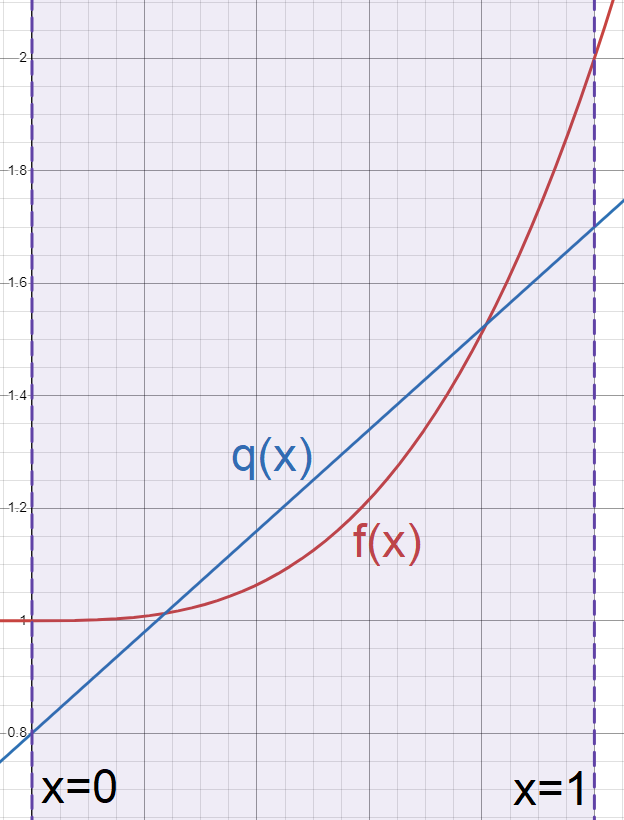
\includegraphics[width=\linewidth]{graph1.png}
    \caption{Wykresy na [0, 1] funkcji\\
    aproksymowanej \textit{f} i aproksymującej \textit{q}.}
\end{wrapfigure}
\vspace{5mm}

\noindent
Podstawiając do układu równań\\
otrzymuję postać

\setstretch{1.25}
\[\left\{
\begin{array}{l}
    c_0 + \frac{1}{2}c_1 = \frac{5}{4}\\
    \frac{1}{2}c_0 + \frac{1}{3}c_1 = \frac{7}{10}
\end{array}
\right.\]

\setstretch{1}
Rozwiązaniem jest:
\setstretch{1.25}

\[\left\{
\begin{array}{l}
    c_0 = \frac{4}{5} = 0.8\\
    c_1 = \frac{9}{10} = 0.9
\end{array}
\right.\]
\setstretch{1}

\noindent
Stąd otrzymujemy wzór\\
funkcji aproksymującej:
\[q(x) = 0.9x + 0.8\]

\clearpage

\subsection{}
Wielomiany Legendre'a \(P_n\) są ortogonalne na przedziale [-1, 1] z wagą 1.\\
Aby uzyskać podobny efekt na zadanym przedziale [0, 1] określam przesunięte wielomiany Legendre'a jako \(\widetilde{P}_n(x) = P_n(2x - 1)\). Poprzez takie przekształcenie afiniczne otrzymujemy wielomiany \(\widetilde{P}_n\) ortogonalne na [0, 1].

\noindent
Szukamy funkcji aproksymującej będącej wielomianem drugiego stopnia, więc skorzystam jedynie z pierwszych trzech przesuniętych wielomianów Legendre'a:
\begin{align*}
    &\widetilde{P}_0(x) = 1\\
    &\widetilde{P}_1(x) = 2x - 1\\
    &\widetilde{P}_2(x) = 6x^2 - 6x + 1
\end{align*}
Ze względu na ortogonalność układu powyższych funkcji współczynniki funkcji aproksymującej są tu określone wzorem
\begin{gather*}
    c_i = \frac{1}{\lambda_i} \int_0^1 \widetilde{P}_i(x) f(x)\ dx, \quad \lambda_i = \int_0^1 \widetilde{P}_i^2(x)\ dx\\
    \text{dla}\ i = 0, 1, 2
\end{gather*}
\begin{wrapfigure}[11]{r}{0.45\textwidth}
    \centering
    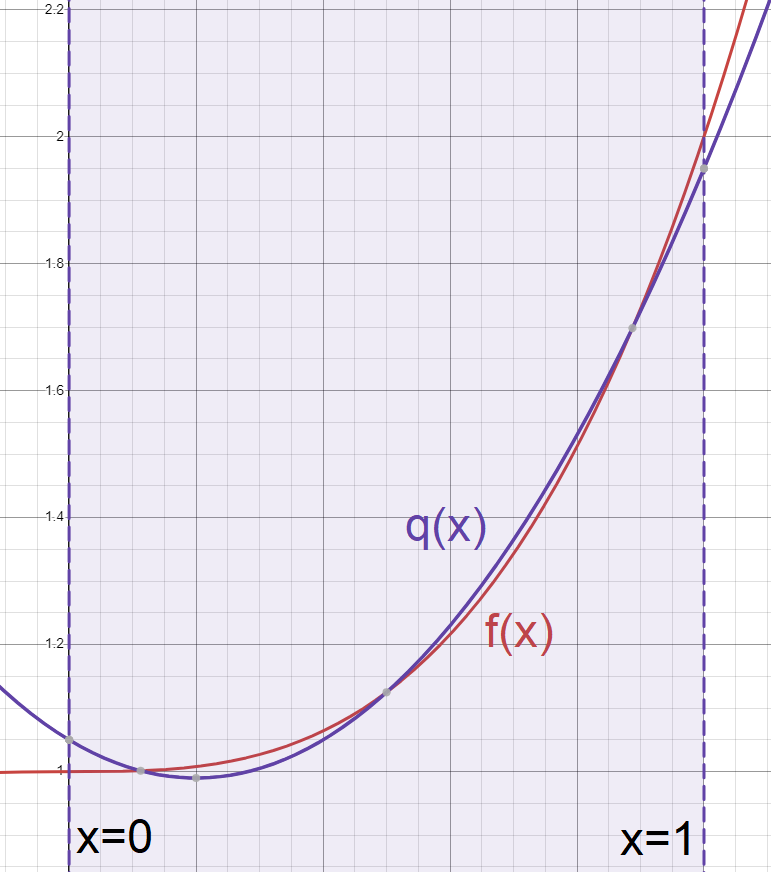
\includegraphics[width=\linewidth]{graph2.png}
    \caption{Wykresy na [0, 1] funkcji aproksymowanej \textit{f} oraz aproksymującej \textit{q}.}
\end{wrapfigure}

\vspace{5mm}
\noindent
Dokonując odpowiednich podstawień\\
uzykuję wyniki:

\setstretch{1.25}
\[\left\{
\begin{array}{l}
    c_0 = \frac{5}{4}\\
    c_1 = \frac{9}{20}\\
    c_2 = \frac{1}{4}
\end{array}
\right.\]
\setstretch{1}

\noindent
Wstawiając te współczynniki do funkcji aproksymującej otrzymuję:
\begin{align*}
    q(x) &= \frac{5}{4} + \frac{9}{20}(2x - 1) + \frac{1}{4}(6x^2 - 6x + 1)\\
    &= \frac{3}{20} (10x^2 - 4x + 7)
\end{align*}

\vspace{15mm}
\noindent
\textbf{Wnioski:} Stopień wielomianu aproksymującego ma ogromne znaczenie dla dokładności aproksymacji, a użycie wielomianów ortogonalnych wyraźnie ułatwia obliczenia.

\clearpage

\section{Rozwiązania zadań domowych}

\subsection{}
\begin{lstlisting}[language=R]
Q <- function(m, x, a_vec) {
  acc <- a_vec[1]
  for (i in 1:m) {
    acc <- acc + a_vec[i+1] * x^i
  }
  return(acc)
}

S <- function(k, n, x_vec) {
  acc <- 1.0
  for (i in 2:n) {
    acc <- acc + x_vec[i]^k
  }
  return(acc)
}

T <- function(k, n, x_vec, y_vec) {
  acc <- 0
  for (i in 1:n) {
    acc <- acc + x_vec[i]^k * y_vec[i]
  }
  return(acc)
}

approximating <- function(x, x_vec, y_vec, m) {
  n <- length(x_vec)
  
  S_mat <- matrix(numeric((m+1)^2), m+1, m+1)
  for (row in 0:m) {
    for (col in 0:m) {
      S_mat[row+1, col+1] <- S(row + col, n, x_vec)
    }
  }
  
  T_vec <- numeric(m+1)
  for (i in 0:m) {
    T_vec[i+1] <- T(i, n, x_vec, y_vec)
  }
  
  a_vec <- solve(S_mat, T_vec)
  return(Q(m, x, a_vec))
}

# przykładowe dane
x_values <- c(1, 2, 5, 7)
y_values <- c(3.2, 2, 2.5, 3.8)
# funkcja jednej zmiennej do rysowania
example <- function(x) {
  return(approximating(x, x_values, y_values, 2))
}
curve(Vectorize(example, 'x')(x),
    min(x_values) - 1, max(x_values) + 1, lwd=2, ylab='y')
points(x_values, y_values, pch=16, col='red')
\end{lstlisting}

\noindent
Powyższy program napisany w języku R realizuje metodę najmniejszych kwadratów aproksymacji punktowej. Główną funkcją jest \verb|approximating|, która reprezentuje funkcję aproksymującą przyjmując jako argumenty:
\begin{itemize}
    \item \verb|x| - argument główny
    \item \verb|x_vec| - wektor odciętych zadanych punktów
    \item \verb|y_vec| - wektor rzędnych
    \item \verb|m| - stopień wielomianu aproksymującego
\end{itemize}
Kod na końcu ilustruje przykładowe użycie tej funkcji, generując poniższy wykres przykładowych punktów i aproksymującej paraboli.

\begin{figure}[h]
    \centering
    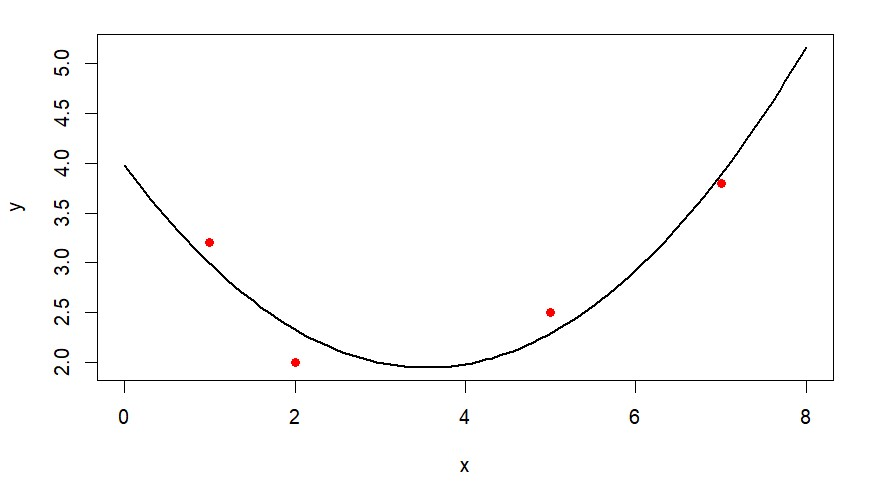
\includegraphics[width=\linewidth]{plot.jpg}
\end{figure}

\newpage

\subsection{}
\begin{table}[h]
    \centering
    \begin{tabular}{c|c|c|c|c|c}
        \(x_i\) & -1 & -0.5 & 0 & 0.5 & 1\\
        \hline
        \(f(x_i)\) & 0 & 0.75 & 1 & 0.75 & 0
    \end{tabular}
    \caption{Wartości funkcji \(f(x) = 1 + x^3\) w zadanych \(n+1=5\) punktach}
    \label{tab:table1}
\end{table}

\noindent
Obliczam kolejne wielomiany Grama do stopnia \(m = 3\) dla \(n = 4\):
\begin{align*}
    F_0(q) &= 1 \hspace{37mm} \text{gdzie } q = 2(x + 1)\\
    F_1(q) &= 1 - 2\frac{q}{n} = 1 - \frac{q}{2}\\
    F_2(q) &= 1 - 6\frac{q}{n} + 6\frac{q(q-1)}{n(n-1)} = \frac{1}{2}(q^2 - 4q + 2)\\
    F_3(q) &= 1 - 12\frac{q}{n} + 30\frac{q(q-1)}{n(n-1)} - 20\frac{q(q-1)(q-2)}{n(n-1)(n-2)}\\
    &= -\frac{5}{6}q^3 + 5q^2 - \frac{43}{6}q + 1
\end{align*}
\begin{table}[h]
    \centering
    \begin{tabular}{c|c|c|c|c|c}
        \textit{q} & \(F_0(q)\) & \(F_1(q)\) & \(F_2(q)\) & \(F_3(q)\)\\
        \hline
        0 & 1 & 1 & 1 & 1\\
        1 & 1 & 0.5 & -0.5 & -2\\
        2 & 1 & 0 & -1 & 0\\
        3 & 1 & -0.5 & -0.5 & 2\\
        4 & 1 & -1 & 1 & -1
    \end{tabular}
    \caption{Wartości funkcji \(F_k\) dla \(q = 0, 1, 2, 3, 4\)}
    \label{tab:table2}
\end{table}

\noindent
Następnie podobnie obliczam odpowiednie \(s_k\):
\begin{align*}
    s_0 &= \sum_{q=0}^4 1^2 = 5\\
    s_1 &= \sum_{q=0}^4 \left(1 - \frac{q}{2}\right)^2 = \frac{5}{2}\\
    s_2 &= \sum_{q=0}^4 \left(\frac{1}{2}(q^2 - 4q + 2)\right)^2 = \frac{7}{2}\\
    s_3 &= \sum_{q=0}^4 \left(-\frac{5}{6}q^3 + 5q^2 - \frac{43}{6}q + 1\right)^2 = 10
\end{align*}
Oraz \(c_k\):
\begin{align*}
    c_0 &= \sum_{q=0}^4 y_i \cdot 1 = \frac{5}{2}\\
    c_1 &= \sum_{q=0}^4 y_i \cdot \left(1 - \frac{x_i}{2}\right) = \frac{5}{2}\\
    c_2 &= \sum_{q=0}^4 y_i \cdot \frac{1}{2}(x_i^2 - 4x_i + 2) = \frac{43}{16}\\
    c_3 &= \sum_{q=0}^4 y_i \cdot \left(-\frac{5}{6}x_i^3 + 5x_i^2 - \frac{43}{6}x_i + 1\right) = \frac{35}{8}
\end{align*}
Można podstawić wyliczone wartości do finalnego wzoru na funkcję aproksymującą:
\[y(x) = \sum_{k=0}^3 \frac{c_k}{s_k} F_k(q), \quad q = 2(x+1)\]
\begin{align*}
    y(x) &= \frac{5}{2} \cdot \frac{1}{5} \cdot 1 + \frac{5}{2} \cdot \frac{2}{5} \cdot \left(1 - \frac{q}{2}\right) + \frac{43}{16} \cdot \frac{2}{7} \cdot \frac{1}{2}(q^2 - 4q + 2) +\\
    &+ \frac{35}{8} \cdot \frac{1}{10} \cdot \left(-\frac{5}{6}q^3 + 5q^2 - \frac{43}{6}q + 1\right) =\\
    &= \frac{1}{2} + 1 - \frac{q}{2} + \frac{43}{112}(q^2 - 4q + 2) + \frac{7}{16} \left(-\frac{5}{6}q^3 + 5q^2 - \frac{43}{6}q + 1\right) =\\
    &= -\frac{35}{96}q^3 + \frac{18}{7}q^2 - \frac{3475}{672}q + \frac{303}{112} = -\frac{35}{12}x^3 + \frac{43}{28}x^2 + \frac{71}{48}x - \frac{15}{56}
\end{align*}

\begin{figure}[H]
    \centering
    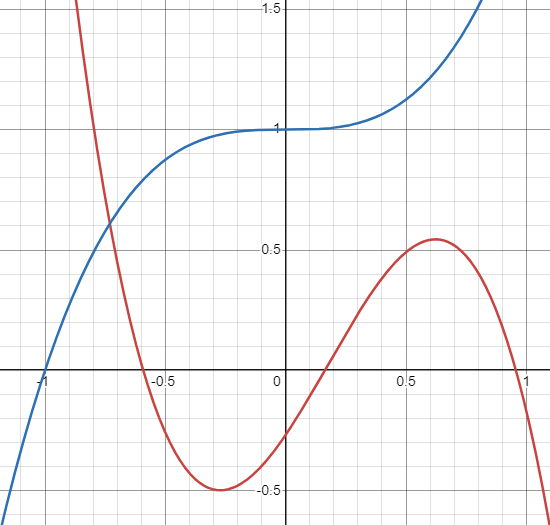
\includegraphics[width=0.48\linewidth]{graph3.png}
    \caption{Porównanie funkcji - gdzieś musiałem popełnić błąd (.\_.)}
\end{figure}

\subsection{}
Funkcja \(f(x) = |\sin x|\) spełnia \href{https://pl.wikipedia.org/wiki/Warunki_Dirichleta}{warunki Dirichleta}, więc ma reprezentację w postaci \href{https://pl.wikipedia.org/wiki/Szereg_Fouriera}{szeregu Fouriera} i można ją rozłożyć na sumę funkcji trygonometrycznych. Jej okresem jest \(\pi\). Trygonometryczny szereg Fouriera jest więc zadany tutaj przez
\begin{align*}
    S(x) &= \frac{a_0}{2} + \sum_{n=1}^{\infty}( a_n \cos(2nx) + b_n \sin(2nx))\\
    a_n &= \frac{2}{\pi} \int_{-\frac{\pi}{2}}^{\frac{\pi}{2}} |\sin x| \cos(2nx)\ dx\\
    b_n &= \frac{2}{\pi} \int_{-\frac{\pi}{2}}^{\frac{\pi}{2}} |\sin x| \sin(2nx)\ dx
\end{align*}
Funkcja \textit{f} jest parzysta, więc współczynnik \(b_n\) jest stale równy 0, bo podcałkowa jest tam nieparzysta. Odwrotnie jest przy \(a_n\), mamy więc:
\[a_n = \frac{2}{\pi} \int_0^{\pi} \sin x \cos(2nx)\ dx = -\frac{4}{\pi(4n^2 - 1)}\]
Stąd ostatecznie
\[S(x) = \frac{2}{\pi} + \frac{4}{\pi} \sum_{n=1}^{\infty} \frac{\cos(2nx)}{4n^2 - 1}\ (= f(x) = |\sin x|)\]
jest sumą tego szeregu. Funkcja \textit{f} może być zatem aproksymowana na zadanym przedziale wybraną sumą częściową:
\[f(x) \approx \frac{2}{\pi} + \frac{4}{\pi} \sum_{k=1}^{N} \frac{\cos(2kx)}{4k^2 - 1}\]

\section{Bibliografia}
Materiały ze strony - Włodzimierz Funika\\
https://en.wikipedia.org/wiki/Legendre\_polynomials\#Shifted\_Legendre\_polynomials\\
https://pl.wikipedia.org/wiki/Szereg\_Fouriera

\end{document}
